\documentclass{beamer}

\mode<presentation> {
	

	\usetheme{Boadilla}
	
	
	\usecolortheme{seagull}  %plain
	
}
\usepackage{subfig}
\usepackage{hyperref}
\usepackage{graphicx} % Allows including images
\usepackage{booktabs} % Allows the use of \toprule, \midrule and \bottomrule in tables

%----------------------------------------------------------------------------------------
%	TITLE PAGE
%----------------------------------------------------------------------------------------

\title[Django Workshop]{Django Workshop Introduction} % The short title appears at the bottom of every slide, the full title is only on the title page

\author{Advanced Programming} % Your name
\institute[AUT] % Your institution as it will appear on the bottom of every slide, may be shorthand to save space
{
	Amirkabir University of Technology\\ % Your institution for the title page
	\medskip
	\textit{} % Your email address
}
\date{Spring 2019} % Date, can be changed to a custom date

\begin{document}
	
	\begin{frame}
		\titlepage % Print the title page as the first slide
	\end{frame}

	\begin{frame}
	\frametitle{Overview} % Table of contents slide, comment this block out to remove it
	\tableofcontents % Throughout your presentation, if you choose to use \section{} and \subsection{} commands, these will automatically be printed on this slide as an overview of your presentation
	\end{frame}

%	PRESENTATION SLIDES

\section{What is Django} 

\begin{frame}
\begin{figure}
	
\includegraphics[width=\linewidth]{Pics/PyDjango.jpg}
\end{figure}
\end{frame}

\begin{frame}
\frametitle{What is Django}
	\centering
	\Large
	free and open-source \color{green}web framework \color{black}
\end{frame}

\begin{frame}
\frametitle{Once upon a time :)}
	\centering
	\large
	Python encourages everyone to code.\\
	Even \color{green}journalists.\color{black}
\end{frame}

\section{Python}
\begin{frame}
\frametitle{Why coding in python?}
\begin{itemize}
	\item large community
	\item less code
\end{itemize}
\begin{figure}
	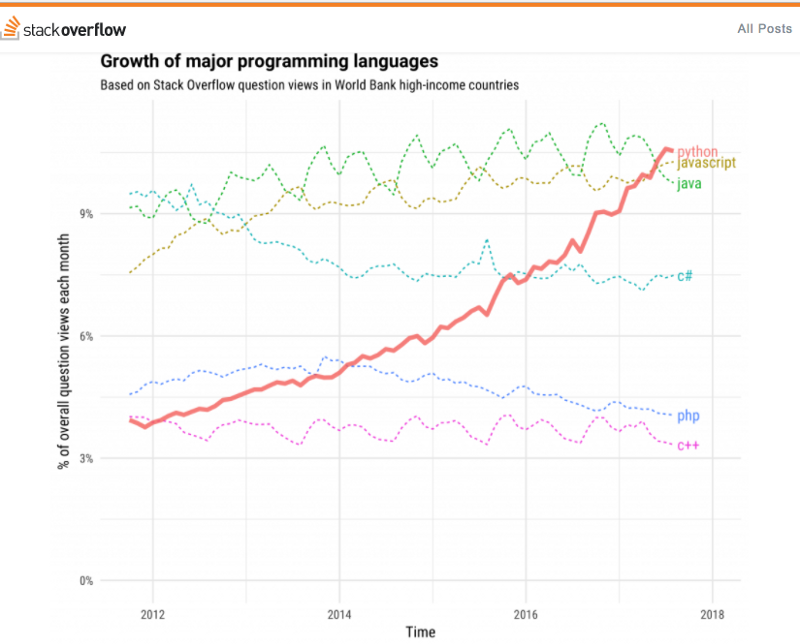
\includegraphics[width=0.6\linewidth]{Pics/python_stack.png}
\end{figure}
\end{frame}

\subsection{Virtual environment}
\begin{frame}
	\frametitle{Virtual environment}
	\begin{figure}
		
\includegraphics[width=\linewidth]{Pics/venv.jpg}
	\end{figure}
\end{frame}

\subsection{Package manager}
\begin{frame}
	\frametitle{install Django on venv}
	\centering
	\Large
	\begin{block}{}
	\$ pip install django\\
	\$ django-admin startproject <name>
	\end{block}
\end{frame}

\begin{frame}
	\begin{figure}
		
\includegraphics[width=0.8\linewidth]{Pics/proj.jpeg}
	\end{figure}
\end{frame}

\begin{frame}
\frametitle{Project files}
	\begin{itemize}
		\item \_\_init\_\_.py
		\item settings.py
		\item urls.py
		\item wsgi.py
		\item manage.py
	\end{itemize}
\end{frame}

\begin{frame}
	\frametitle{Django application}
	\centering
	\Large
	\begin{block}{}
		\$ python manage.py runserver\\
		\$ python manage.py startapp <name>
	\end{block}
\end{frame}

\begin{frame}
\frametitle{Application files}
\begin{itemize}
	\item migrations
	\item \_\_init\_\_.py
	\item admin.py
	\item apps.py
	\item models.py
	\item tests.py
	\item views.py
	\item urls.py
\end{itemize}
\end{frame}

\begin{frame}
	\frametitle{Templates}
	\begin{itemize}
		\item templates directory
		\item add it in settings
	\end{itemize}
\end{frame}

\begin{frame}
\begin{figure}
	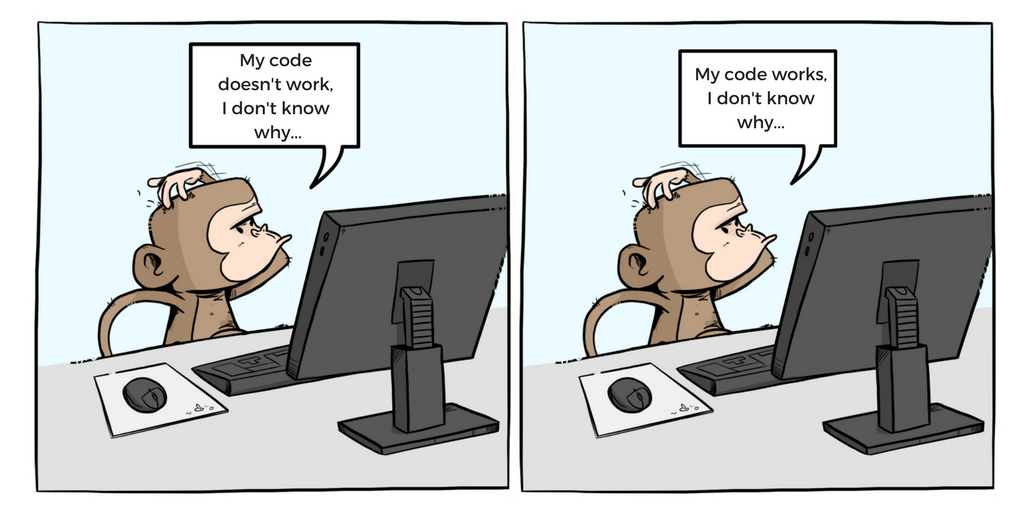
\includegraphics[width=0.8\linewidth]{Pics/why.png}
\end{figure}
\end{frame}

\begin{frame}
\frametitle{What about static files}
\begin{figure}
	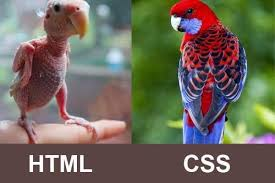
\includegraphics[width=0.6\linewidth]{Pics/css.jpeg}
\end{figure}
\end{frame}

\begin{frame}
	\frametitle{Database}
	\begin{itemize}
		\centering
		\large
		\item classes for tables
		\item attributes for columns
		\item instances for records		
	\end{itemize}
\end{frame}

\section{MTV}
\begin{frame}
\frametitle{What is MTV?}

\begin{figure}
	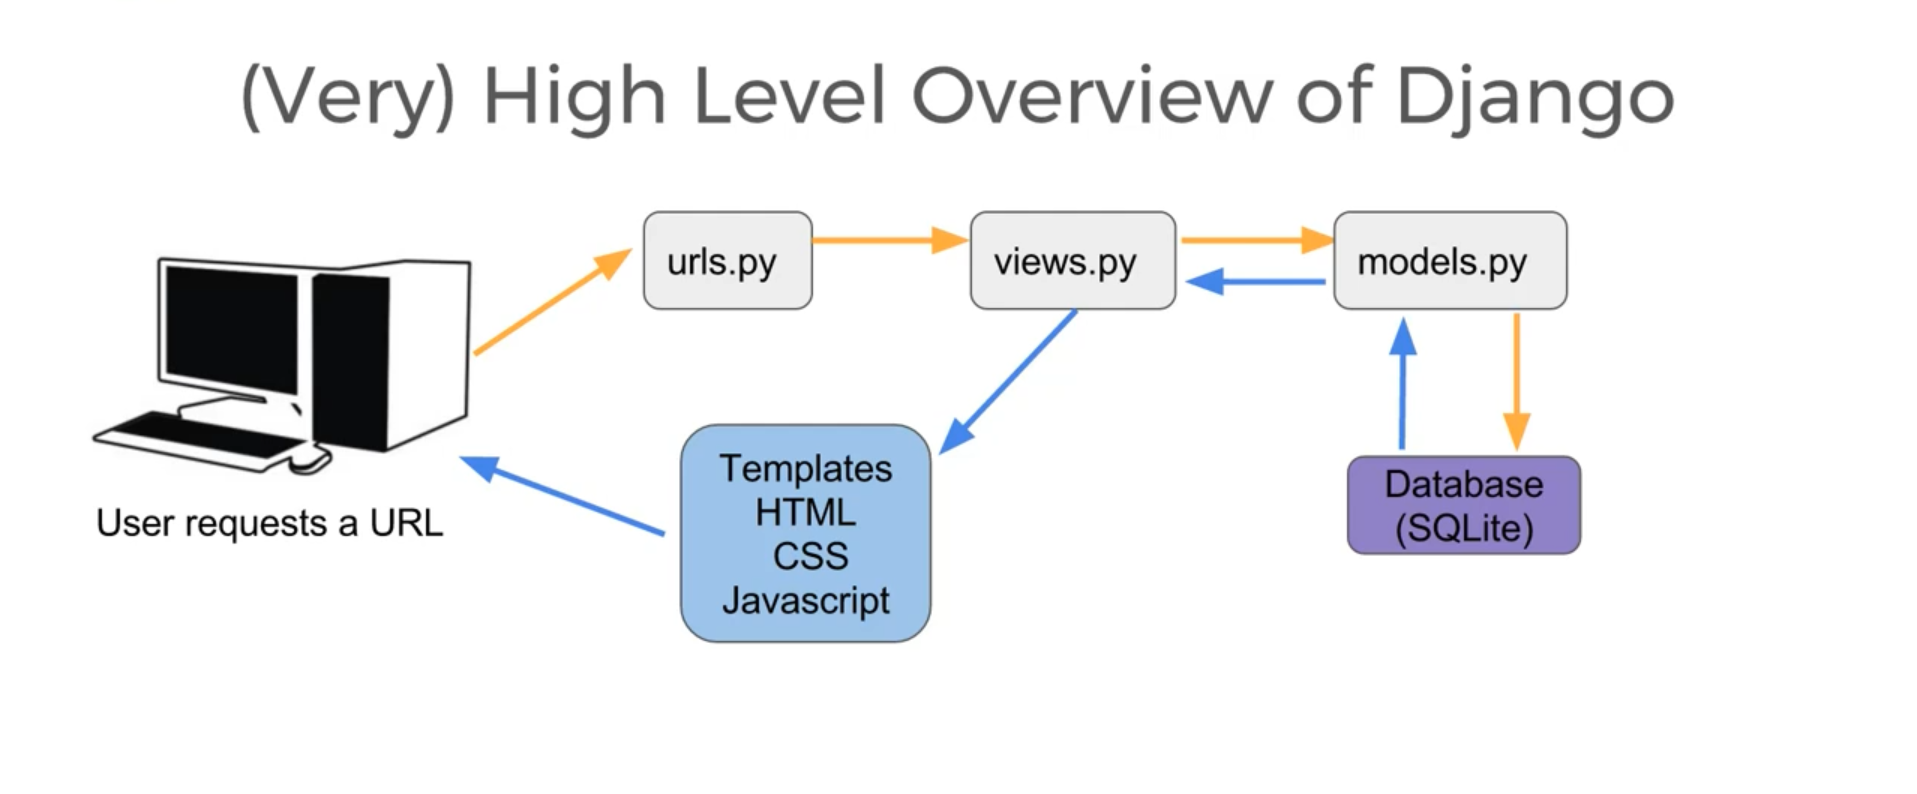
\includegraphics[width=\linewidth]{Pics/High_level.png}
\end{figure}
\end{frame}

\begin{frame}
\frametitle{What is MTV?}

\begin{block}
	
	\begin{itemize}
		\item "M"odel : data layer. $\rightarrow$ models.py 
		\item "T"emplate : presentation layer. $\rightarrow$ templates/
		\item "V"iew : business logic layer. $\rightarrow$ views.py 
		
	\end{itemize}
\end{block}
\end{frame}

\begin{frame}
	\frametitle{Forms: user inputs}
	\begin{itemize}
		\centering
		\large
		\item forms.py
		\item similar to models
	\end{itemize}
\end{frame}

\begin{frame}
	\frametitle{Simpler urls}
	\begin{itemize}
		\centering
		\large
		\item app\_name in urls.py
		\item relative url in href
	\end{itemize}
\end{frame}

\begin{frame}
\frametitle{Inheritance in templates}
\begin{itemize}
	\centering
	\large
	\item create base.html
	\item make blocks in base file
	\item use extend in child file
\end{itemize}
\end{frame}


\section{Django in real world}
\begin{frame}	
	\begin{figure}
		\centering
		\subfloat[instagram]{
\includegraphics[width=0.5\textwidth]{Pics/insta.png}}
		\subfloat[spotify]{
\includegraphics[width=0.5\textwidth]{Pics/spotify.png}}
	\end{figure}
\end{frame}

\begin{frame}	
\begin{figure}
	\centering
	\subfloat[mozilla]{
\includegraphics[width=0.5\textwidth]{Pics/mozilla.jpeg}}
	\subfloat[dropbox]{
\includegraphics[width=0.5\textwidth]{Pics/dropbox.jpg}}
\end{figure}
\end{frame}

\begin{frame}	
\begin{figure}
	\centering
	\subfloat[youtube]{
\includegraphics[width=0.5\textwidth]{Pics/youtube.png}}
	\subfloat[pinterest]{
\includegraphics[width=0.4\textwidth]{Pics/pin.png}}
\end{figure}
\end{frame}

\begin{frame}
	\frametitle{What next?}
	\begin{itemize}
		\centering
		\large
		\item Blog project
		\item Social network project
	\end{itemize}
\end{frame}

\begin{frame}
\frametitle{References}
	\href{https://en.wikipedia.org/wiki/Django_(web_framework)}{https://en.wikipedia.org/wiki/Django-(web-framework)}
	\href{https://www.djangoproject.com/}{https://www.djangoproject.com/}
\end{frame}

\begin{frame}
\begin{figure}
	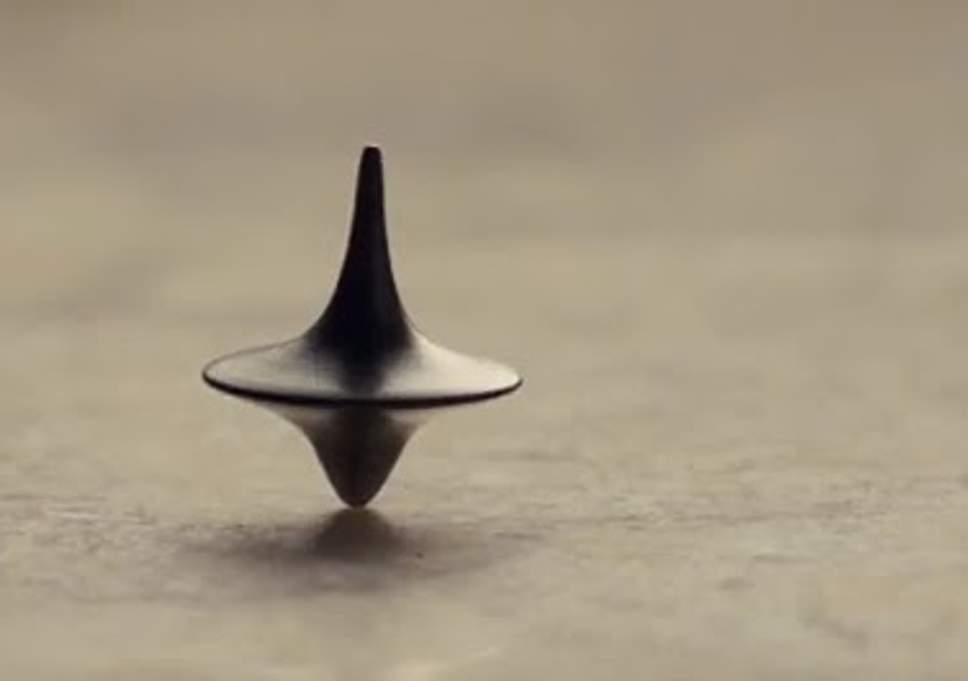
\includegraphics[width=0.8\linewidth]{Pics/end.jpg}
\end{figure}

\Huge
\centering
The End
\end{frame}

\end{document} 